\begin{figure}[t]
	\centering
	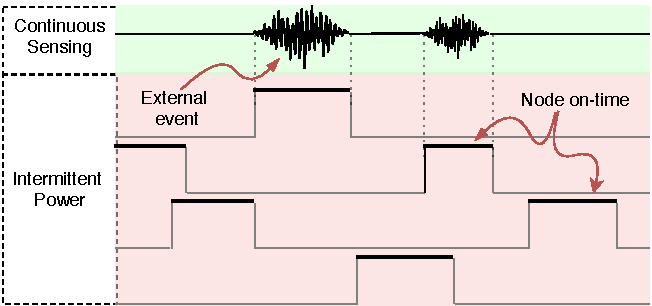
\includegraphics[width=\columnwidth]{figures/coalInterSen}
	\caption{A \fullsys (\sys) is a group of intermittently-powered nodes that sense continuously despite the intermittent power supply. \sys exploits the inherent randomization of energy harvesting systems, if available, and introduces artificial randomization to preserve continuous sensing when needed.}
	\label{fig:powerCycle}
\end{figure}
%
The vision of smart cities, through the use of Internet of Things technologies, requires billions of sensors providing the necessary context to aid people in their daily lives. For example, cars will no longer need to wait in front of traffic lights for non-existing pedestrians to cross the road; doors, upon leaving, will provide people with the latest weather forecast; and jackets will adjust air circulation based on body temperature. 

Unfortunately, batteries do not provide a viable solution to power all the needed sensors in smart cities. Batteries can be bulky, for example, 32\% of a $\SI{1}{g}$ sensing "backpack" fixed on a cyborg insect is a battery~\cite{daly2010pulsed}; hazardous; and expensive---they will deplete and require maintenance leading to service disruptions and heightened subscription fees. Moreover, the raw materials for making batteries are also limited. Therefore, future sensors must leave batteries behind and rely on green, perpetual energy sources. 

Natural energy sources such as light, vibration, and heat can power tiny sensors directly~\cite{margolies2016panda, gorlatova2014movers, gorlatova2010energy, gollakota2014emergence}. Tiny energy harvesters, however, can only scavenge a very limited power from such energy sources~\cite{liu2013ambient}. Therefore, an energy-harvesting sensor operates intermittently. An intermittent sensor starts by harvesting a certain amount of energy in its buffer (i.e., a super-capacitor). Subsequently, it triggers operation which depletes the buffered energy quickly, as the power consumption rate tends to be much higher than the power accumulation rate. Once the energy is below a certain level, the sensor experience a complete power-down, the cycle of charging and operating %continues indefinitely
repeats~\cite{colin2018reconfigurable}.

%\textcolor{red}{\bf Stephan": trade-off or exchange?}
Intermittent devices trade off a reliable energy source (the battery) for a sustainable
%--- when a large number of sensors are considered --- 
energy source, i.e., ambient energy. This switch to energy harvesting generates many challenges~\cite{lucia2017intermittent}. For example, preserving computation progress under frequent power interrupts, enabling timely operations with indeterminate power-down duration, and the fact that nodes operate intermittently. 

Researchers continue to investigate these challenges. For example, \cite{lucia2017intermittent,mementos,dino,colin2016chain,balsamo2015hibernus} studied the intermittent computation problem, which is concerned with the preservation of an application progress and data consistency under frequent power failures; \cite{hester2017timely} investigated the timely operation challenge, which is concerned with data freshness after a power interrupt; \cite{samoyed_pldi_2019} introduced a system design for peripherals states preservation for intermittently powered sensors;  and \cite{yildirim2018ink} introduced event-driven execution for the intermittent domain, which deals with input and output operations under arbitrarily-timed power loss.

Despite significant progress achieved in the intermittent domain, \textit{the system availability problem} has not been addressed. A monitoring sensor that has a very low probability to be available when an external event occurs is not worth deploying. A sensor that is capable of capturing only very short events has a limited number of potential applications. 
For example, a voice-controlled light-switch capable of only accepting short (single-word) commands has its limitations. Using "on" to turn on the lights might turn on other devices as well. Using "lights" does not allow the specification of "on" or "off". Consequently, intermittent sensors have not gained widespread adoption.

This paper tackles the paradox of continuous sensing on intermittent devices. It studies the randomized power cycle of energy-harvesting platforms and makes a key observation about the inter-relationship between these platforms. Sensors driven by the same ambient energy source (e.g., light or RF) do {\em not} show correlated on/off (sense/charge) cycles. Building on top of this observation, the paper introduces a new type of sensor that we call \textit{\fullsys} (\sys). The \sys is defined as the abstraction of a group of energy-aware intermittent nodes providing the collective sense of being always on. Figure~\ref{fig:powerCycle} illustrates the \sys concept for our prototype implementation of a command recognizer; a number of solar-powered nodes equipped with a microphone recording voice commands in a smart home setting. Recording and processing a word depletes the super capacitor powering a node, ``silencing'' it until the subsequent recharging completes. Multiple nodes with (partially overlapping) on/off cycles spread in time can provide continuous service despite the inherent intermittency.

In contrast to periodic (one-shot) sensing applications, event-based applications (like our command recognizer) may induce implicit synchronization (multiple nodes detecting the same command) that compromises the availability required by the application (all node recharge after the first word, missing any subsequent word). To guarantee continuous availability, a \sys may need to introduce artificial randomness. Doing so, however, is non-trivial as knowledge is needed about the number of (charged) nodes, which depends on a number of factors including environmental conditions regarding the power source (e.g., light intensity). This paper provides an estimator based on local measurements of a node's duty cycle that has been used effectively on our prototype command recognizer enabling it to detect commands of four words with above 90\% detection accuracy. 
In summary this paper makes the following contributions:
\begin{itemize}
		\item We introduce a new type of sensor that is an intermittently powered, yet senses continuously. The \textit{\fullsys} (\sys) is the abstraction of a group of intermittently-powered sensors exploiting (inherent) randomization to spread awake times uniformly.
		\item We model the (\sys) availability of energy-harvesting nodes and validate it against in-the-wild measured data and under controllable energy conditions.   
		\item We introduce an algorithm for a node to determine its own duty cycle, which depends on the ambient power source. That duty cycle can effectively be used to estimate the number of active neighbors, which in turn decides if a node should back off to avoid duplicate event detection and availability interruptions (implicit synchronization in favourable harvesting conditions).
		\item We prototype, evaluate, and demonstrate the feasibility of the \fullsys concept in the form of voice-control application recognizing individual words on solar-powered nodes equipped with a microphone.
\end{itemize}

%\todo{Potential applications, relocate to the appreciated location}
%For example, once a certain on/off cycle is preserved, an intermittent wake-up receiver can be implemented; an intermittent acoustic monitoring system for monitoring engines modules---the sound produced by a deformed gear tooth---can be made. Moreover, with the advances in passive communication (such as passive light~\cite{}, and backscatter tag-to-tag~\cite{liu2013ambient} communication) battery-free miniaturized sensors can form self-powered wireless sensor network to, for instance, create smart wallpaper and revolutionize smart buildings.